% XCircuit output "rf.tex" for LaTeX input from rf.eps
\def\putbox#1#2#3#4{\makebox[0in][l]{\makebox[#1][l]{}\raisebox{\baselineskip}[0in][0in]{\raisebox{#2}[0in][0in]{\scalebox{#3}{#4}}}}}
\def\rightbox#1{\makebox[0in][r]{#1}}
\def\centbox#1{\makebox[0in]{#1}}
\def\topbox#1{\raisebox{-0.60\baselineskip}[0in][0in]{#1}}
\def\midbox#1{\raisebox{-0.20\baselineskip}[0in][0in]{#1}}
   \scalebox{1}{
   \normalsize
   \parbox{5.75521in}{
   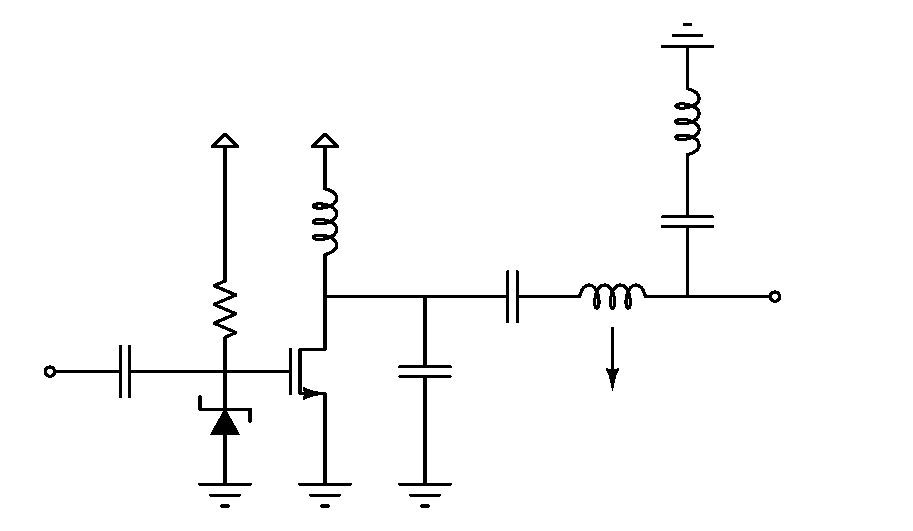
\includegraphics[scale=1]{rf}\\
   % translate x=896 y=364 scale 0.38
   \putbox{0.06in}{1.04in}{1.20}{$P_{in}$}%
   \putbox{4.89in}{1.54in}{1.20}{$P_{out}$}%
   \putbox{4.64in}{2.54in}{1.20}{$L_h$}%
   \putbox{4.72in}{1.87in}{1.20}{$C_h$}%
   \putbox{3.22in}{1.70in}{1.20}{$C_s$}%
   \putbox{3.89in}{1.70in}{1.20}{$L_s$}%
   \putbox{2.97in}{0.87in}{1.20}{$C_p$}%
   \putbox{2.22in}{1.87in}{1.20}{RFC}%
   \putbox{0.89in}{0.54in}{1.20}{$D_1$}%
   \putbox{2.06in}{0.87in}{1.20}{$M_1$}%
   \putbox{0.64in}{1.20in}{1.20}{$C_i$}%
   \putbox{1.56in}{1.29in}{1.20}{$R_i$}%
   \putbox{1.31in}{2.62in}{1.20}{$V_{dd}$}%
   \putbox{1.97in}{2.62in}{1.20}{$V_{dd}$}%
   \putbox{3.56in}{0.62in}{1.20}{HIGH-Q}%
   \putbox{3.39in}{0.37in}{1.20}{INDUCTOR}%
   } % close 'parbox'
   } % close 'scalebox'
   \vspace{-\baselineskip} % this is not necessary, but looks better
